\documentclass[a4paper,12pt]{article}

\usepackage[
    pdftex,
    pdftitle={CGPACK manual},
    pdfauthor={Joe Phillips, Anton Shterenlikht, University of Bristol},
    pdfpagemode={UseOutlines},
    pdfpagelayout={TwoColumnRight},
    bookmarks, bookmarksopen,bookmarksnumbered={True},
    pdfstartview={FitH},
    colorlinks, linkcolor={blue}, citecolor={blue}, urlcolor={blue}
    ]{hyperref}

\usepackage{amssymb, amsmath, amsthm, eulervm, multicol, comment}
\usepackage{natbib,graphicx}

\usepackage[lined,boxed,linesnumbered]{algorithm2e}

\setcounter{tocdepth}{1}

\title{CGCA manual}

\author{A Shterenlikht, J Phillips \\
Mech Eng Dept, University of Bristol, UK}

\begin{document}

\newcommand{\tenrtwo}[1]{\mathbold{#1}}
\newcommand{\tenrfour}[1]{\mathcal{#1}}

\maketitle

\tableofcontents

\section{Conventions}
\label{sec:conventions}

Italic is used for scalars and vectors: {\em{$p$}}, $q$.
It is easy to distinguish which are which by context.
Bold maths is used for rank 2 tensors:
$\tenrtwo{I}$,
$\tenrtwo{R}$,
$\tenrtwo{\sigma}$.
Script is used for rank 4 tensors:
$\tenrfour{C}$.

`$\cdot$' denotes dot product, single contraction:
$x^s=\mathbold{R}^c \cdot x^c$.

`:' denotes double product, double contraction:
$\tenrtwo{\sigma} = \tenrfour{C} : \tenrtwo{\epsilon}$.

`$\otimes$' denotes tensor product:
$\mathbold{I}\otimes\mathbold{I}=
\delta_{ij}\delta_{kl}$.

\subsection{Space coarray}
\label{sec:space:coarray}

The space coarray is the centre part of the whole
library.
The idea is that 3D space is partitioned into identical
cells of some sort.
The cells are used to store and update some physically
relevant properties.
An important consideration is how many properties can
a cell store.
At present the coarray is defined as shown in
Eqn. \eqref{eq:coarray}:

\begin{equation}
\texttt{
coarray(l1:u1,l2:u2,l3:u3,props)[col1:cou1,col2:cou2,col3:*]
}
\label{eq:coarray}
\end{equation}
%
where \texttt{l1}\ldots\texttt{u3}
are the lower and the upper
spatial bounds of the array, counted in cells;
\texttt{props} is the number of properties a cell should
hold; \texttt{col1}\ldots\texttt{col3} are the lower
and the upper cobounds of the coarray.
Note that the last codimension is never specified,
i.e. it is always left as an asterix, \texttt{*}, to
allow for different number of images at runtime.

A typical definition of the coarray might look like

\begin{equation}
\texttt{
coarray(1:10,1:10,1:10,2)[1:8,1:8,1:*]
}
\nonumber
\end{equation}
%
which, when run on 512 images, will have the final
codimension of 8.
This array has 2 cell state types, which can be e.g.
the (unique) grain number, and a possible fracture state.

The library has two state types defined:
\texttt{cgca\_state\_type\_grain} for grain states,
i.e. grain numbers, and
\texttt{cgca\_state\_type\_frac} for fracture states.
So \texttt{coarray(:,:,:,cgca\_state\_type\_grain)} is
the local grain array, and
\texttt{coarray(:,:,:,cgca\_state\_type\_frac)} is
the local fracture array.

\subsection{Cellular neighbourhood}

We use a square 3D cellular array.
This means that a cell has a
$3 \times 3 \times 3 - 1 = 26$
cell nearest neighbourhood.
There are a number of problems with such
neighbourhood.
Not all neighbouring cells are `equal'.
If one imagines a $3\times 3 \times 3$ cube
of cubic cells, then the central cell will
have 6 neighbours sharing a face with it,
12 neighbours sharing an edge and 8 neighbours
sharing an edge.
More importantly, there are
three distinct angles between the pairs of the
nearest neighbourhood vectors, i.e. vectors
connecting the centres of the central cell,
and of each neighbouring cell \cite{shterenlikht2013c}.

Perhaps a better idea of a neighbourhood can
be constructed by imagining the central cell
as a 26-faced polyhedra.
Examples are rhombicuboctahedron or
pseudo-rhombicuboctahedron, also called
elongated square gyrobicupola, Johnson solid
J37, see Fig. \ref{fig:j37}.

\begin{figure}
\begin{tabular}{cc}
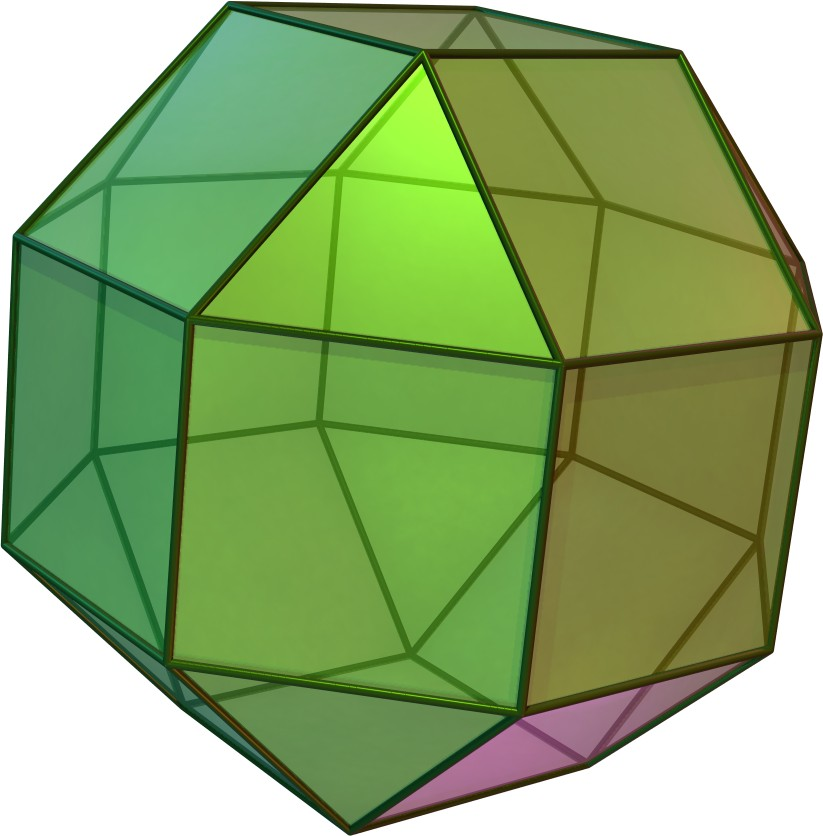
\includegraphics[width=0.4\textwidth]{./Rhombicuboctahedron.png}
&
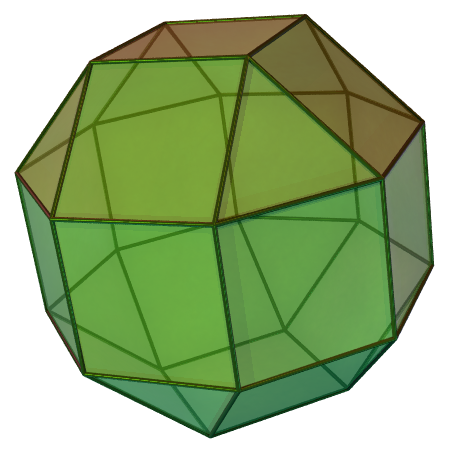
\includegraphics[width=0.4\textwidth]{./Elongated_square_gyrobicupola.png}
\\
(a) & (b)
\end{tabular}
\caption{
26-face polyhedra: (a) Rhombicuboctahedron, an Archimedian
solid, (b) Elongated square gyrobicupola, or
pseudo-rhombicuboctahedron, Johnson solid, J37.
From: http://en.wikipedia.org/wiki/Rhombicuboctahedron and
http://en.wikipedia.org/wiki/Elongated\_square\_gyrobicupola.
}
\label{fig:j37}
\end{figure}

Importantly, the cell state is determined
by the states of its neighbours, not the
other way round.
This helps develop a parallel model using
halo arrays.


\section{\texttt{CG\_CLVG}: cleavage propagation
through CA array}

\label{sec:cg_clvg}

\subsection{Purpose}

The aim of this routine is to propagate a cleavage
crack through the CA array.

\subsection{See also}

\hyperref[sec:cg_cpp]{\texttt{CG\_CPP}} 

\subsection{Interface}

\begin{verbatim}

! IN: ITERS - INTEGER, HOW MANY ITERATIONS OF FRACTURE PROPAGATION TO DO
!       SP1 - REAL, MAX PRINCIPAL STRESS VALUE
!       SPV - VECTOR IN THE DIRECTION OF THE MAX PRINCIPAL STRESS
!   SLFSMLR - IF .TRUE., ENFORCE SELF-SIMILAR BOUNDARY CONDITIONS
!     DEBUG - LOGICAL. IF .TRUE., WILL DUMP *LOTS* OF DEBUG OUTPUT
! OUT: ERRSTAT - 0 IF SUCCESS, NON-ZERO IF A PROBLEM
!  
!**********************************************************************73
!  
! ONELINE: TRANSGRANULAR CLEAVAGE PROPAGATION
!     
!**********************************************************************73
 
 SUBROUTINE CG_CLVG(ITERS,SP1,SPV,SLFSMLR,DEBUG,ERRSTAT)

 USE CG_MOD
 IMPLICIT NONE

 INTEGER,INTENT(IN) :: ITERS
 REAL(KIND=8),INTENT(IN) :: SP1,SPV(3)
 LOGICAL,INTENT(IN) :: SLFSMLR,DEBUG
 INTEGER,INTENT(OUT) :: ERRSTAT

\end{verbatim}

\subsection{Details}

We base our ideas on fracture on books like \cite{averbach1959}

The basic ideas are:

\begin{itemize}

\item

Just as with solidification, scan through alive (un-fractured cells).

\item

A crack will grow when alive cell will acquire state ``fractured''.

\item

There must be a distinction between crack front, which can grow,
and crack flanks, which can't grow.

\item

The process must be probabilistic, with the probability of cleavage
propagating depending on the direction of the maximum principal
stress, and the location within the crack (front vs flanks).

\end{itemize}

These ideas lead to the cleavage modelling flowchart, shown
in Fig. \ref{fig:cl:fc}

\begin{figure}[htb]
\centering
\includegraphics[height=0.9\textheight]{./cleavage-fc.pdf}
\caption{Flowchart of cleavage modelling in
\hyperref[sec:cg_clvg]{\texttt{CG\_CLVG}} 
.}
\label{fig:cl:fc}
\end{figure}

We now describe the flowchart from top to bottom.

Scan through all cells in a CA array. $i$ is the index of the
current cell. At \texttt{START} of each iteration, increment $i$.
If $i>N$, where $N$ is the total number of cells in the array,
then there are no more cells, so this is the \texttt{END} of the process. 

If $i\le N$, then make sure cell $i$ is alive (remember we scan
through alive cells!). If not, then get back to the beginning
and start next iteration, increment $i$.

If cell $i$ is alive,
then make sure it's at the crack flank.
We use a number of neighbouring failed cells as the criterion
for this. The idea is that alive cell touching a crack front
will have few failed cells. When alive cell touches crack
flank, it will have lots of failed cells. At present we set
the threshold at 8 failed cells. This is based on a $3\times3=9$ cell
square - one plane of a $3\times 3 \times 3$ neighbourhood.
If alive cell is touching a crack flank, it is likely to 
have $\geq 9$ failed neighbours.

If cell $i$ is not at crack tip, go to the beginning, increment
$i$, and start next iteration.

Randomly choose a failed cell $j$ from the neighbourhood of cell $i$.
(Note that in solidification we did not worry about a specific
state of a neighbouring cell. However, the physical origins of
cleavage lead to the idea that, once started to propagate, a fast running
cleavage crack is extremely likely to continue to run, until
the catastrophic fracture results, or until the crack driving
force falls dramatically. This means we don't want to allow
copying of ``alive'' to ``alive'', because this will slow
down the propagation rate and will make modelling of cleavage
propagation at real time speeds hard.)

Once a failed cell $j$ has been identified, calculate
the unit vector from $i$ to $j$, let's call it $\vec{a}$.

Then do a dot product of $\vec{a}$ and the unit vector
showing the direction of the maximum principal stress,
$\vec{n}$. The dot product is 1 if the vectors are parallel,
and 0 if they are normal. This means we can use
$1-\texttt{dot product}(a,n)$ as a probability of cleavage.
The probability is high if the dot product is close
to 0, and low if the dot product is close to 1.

The curve is shown in Fig. \ref{fig:cl:prob}

\begin{figure}[htb]
\centering
\includegraphics[width=1.3\textwidth]{./cleavage1.pdf}
\caption{Probability of cleavage as a function of the
dot product of the normal vector and the direction vector for
the chosen cell, $n\cdot a$. Factor $N$ is varied from
1 to 10, with the highest $N$ giving the highest gradient.}
\label{fig:cl:prob}
\end{figure}

We take another random number, \texttt{RND}, in the interval [0\ldots 1).
Finally we check that  $1-\texttt{dot product}(a,n) < \texttt{RND}$.
If true, then cell $i$ becomes ``failed''.
Looking at Fig. \ref{fig:cl:prob} an angle of 80$^\circ$
gives $>80$\% probability of cleavage; an angle of 60$^\circ$
degrees gives about 50\% probability of cleavage; and for
an angle of 40$^\circ$ the probability of cleavage
drops to about 20\%. Of course, the shape of this curve,
and therefore the probabilities, can be changed in future.

Then new iteration starts.

\section{\texttt{CG\_CPP}:
 calculation of the minimum angle (maximum projection)
 between a vector in a CA coord. system and a crystal
 vector}

\label{sec:cg_cpp}

\subsection{Purpose}

The aim of this routine is to find a crystallographic
direction (or a crystallographic plane having this
direction as a normal)
that is closest to the direction of the
applied vector in CA coord. system. If the applied
vector is the direction of the maximum principal
stress, then this plane is a candidate for cleavage
propagation.

\subsection{See also}

\hyperref[sec:cg_clvg]{\texttt{CG\_CLVG}},
\hyperref[sec:cg_csym]{\texttt{CG\_CSYM}}

\subsection{Interface}

\begin{verbatim}

! IN:
!        AVEC - A VECTOR IN CA COORD. SYSTEM
!           R - ROTATION TENSOR, DEFINING THE ORIENTATION OF A CRYSTAL
!        CVEC - CRYSTAL VECTOR, IN CRYSTAL COORD. SYSTEM
! OUT:
!     MAXPROJ - MAX PROJECTION OF THE AVEC ONTO CVEC AND ALL OTHER
!               CRYSTAL VECTORS DEFINING PLANES OF THE SAME FAMILY
!               AS CVEC.
!         CCA - THE CRYSTAL VECTOR IN CA COORD. SYSTEM, WHICH
!               PRODUCES THE MAX PROJ VALUE.
!
!**********************************************************************73
!
! ONELINE: MIN ANGLE BETWEEN A VECTOR AND A NORMAL TO A CRYSTAL PLANE
!
!**********************************************************************73

 SUBROUTINE CG_CPP(AVEC,R,CVEC,MAXPROJ,CCA)

 IMPLICIT NONE

 REAL(KIND=8),INTENT(IN) :: AVEC(3),R(3,3),CVEC(3)
 REAL(KIND=8),INTENT(OUT) :: MAXPROJ,CCA(3)

\end{verbatim}

\subsection{Details}

This routine is non-trivial only because of the
need to take crystal symmetry into account. Refer
to Fig. \ref{fig:cg_cpp} below.

\begin{figure}[htb]
\centering
\includegraphics[width=0.5\textwidth]{./cg_cpp.pdf}
\caption{Schematic diagram illustrating
\hyperref[sec:cg_cpp]{\texttt{CG\_CPP}}
routine. Refer to the main text for details.}
\label{fig:cg_cpp}
\end{figure}

Consider a CA array with its coord. system (superscript
CA). A vector $\vec{a}$ is defined in this coord. system.

Within the CA array there is a grain (crystal) defined by
its rotation tensor $\mathbf{R}$, which has the usual
meaning: a vector $\vec{c}$ in the crystal coord. system
is transformed into a vector in the CA coord. system as

\begin{equation}
 c^{CA}
  =
   \mathbf{R} c^{C}
 \label{eq:cpp:pub}
\end{equation}
%
where superscript $C$ means relative to the crystal
coord. system.

Both $\vec{a}$ and $\vec{c}$ are unit vectors.

The dot product of $\vec{a}$ and $\vec{c}$ is
obtained simply as (in tensor notation)

\begin{equation}
 \texttt{dot product }
  =
   a\cdot\mathbf{R}c
 \label{eq:cpp:pluck}
\end{equation}

However, due to crystal symmetry, $\vec{c}$ defines
a class of planes, not just one plane. To take this into
account we use rotational symmetry tensors, $\mathbf{R}^S$,
see \hyperref[sec:cg_csym]{\texttt{CG\_CSYM}}.
For cubic crystals there are 24 distinct $\mathbf{R}^S$
tensors, including the trivial $\mathbf{R=I}$.

So we get 24 dot products, of which we choose
the one with the maximum absolute value
for output

\begin{equation}
 \texttt{max dot product }
  =
   \max
    |
     a \cdot \mathbf{R} \mathbf{R}^S c
    |
 \label{eq:cpp:mumps}
\end{equation}

The rotational symmetry
tensor, producing the maximum dot product value,
$\mathbf{R}^S_{max}$ is used to calculate the
crystallographic plane, of type defined by $\vec{c}$,
that is closest to being normal to $\vec{a}$:
$\mathbf{R}^S_{max}c$.


\section{\texttt{CG\_CSYM}:
 return on demand a crystal rotation symmetry tensor}

\label{sec:cg_csym}

\subsection{Purpose}

Crystal rotation symmetry must be taken into
account in many routines. This routine stores
24 rotation symmetry tensors and returns one
on demand. Note that the indentity tensor is
one of the 24. So there are 23 non-trivial
rotation symmetry tensors.

\subsection{See also}

\hyperref[sec:cg_cpp]{\texttt{CG\_CPP}}

\subsection{Interface}

\begin{verbatim}

!  IN: NUM - INTEGER, ROTATION SYMMETRY TENSOR NUMBER
! OUT:  RS - REAL, ROTATION SYMMETRY TENSOR
! 
!**********************************************************************73
! 
! ONELINE: RETURNS ONE OF 24 CUBIC SYMMETRY ROTATION TENSORS
! 
!**********************************************************************73

SUBROUTINE CG_CSYM(NUM,RS)

 IMPLICIT NONE

 INTEGER,INTENT(IN) :: NUM
 REAL(KIND=8),INTENT(OUT) :: RS(3,3)

\end{verbatim}

\subsection{Details}

A good introduction is given in \cite{engler2010}.

\section{Cleavage algorithm}

A grain (crystal) is described by its rotation
tensor, $\tenrtwo{R}^c$, with the usual meaning:
a vector in the crystal coord. system, $x^c$,
is transformed into a vector in spatial (cellular) coord. system,
$x^s$, as

\begin{equation}
 x^{s}
  =
   \tenrtwo{R}^{c} \cdot x^{c}
 \label{eq:cgca:pub}
\end{equation}

It is assumed that the cleavage is controlled by
$\sigma_1$, the max principal stress.
If $\sigma_1^s$ is the max principal stress vector
in the spatial coord. system, then
$\sigma_{1}^{c} = \tenrtwo{R}^{s} \cdot \sigma_{1}^{s}$
is the max principal stress vector in the crystal
coord. system.
Here:

\begin{equation}
 \tenrtwo{R}^{s}
 \equiv
 \tenrtwo{R}^{-c}
  \equiv
   \left (
           \tenrtwo{R}^{c}
   \right)^{-1}
    \equiv
     \left (
             \tenrtwo{R}^{c}
     \right)^{T}
\label{eq:cgca:wonk}
\end{equation}

Each crystal plane, \{hkl\}, has a partucular
surface energy, $\gamma_{hkl}$.
We postulate that the work of cleavage
is equal to the surface energy.
The work of cleavage is $\sigma_{hkl}$ times the distance necessary
to break the atomic bonds.
Following the ideas of \cite{gilman1959},
we take this distance equal to $a_0$, the
relaxation distance, which is the atom
diameter in the cleavage plane.
So the cleavage condition will be

\begin{equation}
 \sigma_{hkl}
   a_0
    =
     \gamma_{hkl}
\label{eq:cleav}
\end{equation}

from which the stress required to
cleave \{hkl\} plane is

\begin{equation}
 \sigma_{hkl}
  =
   \frac{ \gamma_{hkl}} { a_0}
\label{eq:muk}
\end{equation}

From \cite{gilman1959}, $\gamma_{100}$=1440,
$\gamma_{110}$=1710 and $\gamma_{111}$=5340erg/cm$^2$
(1erg/cm$^2$ = 10$^{-3}$J/m$^2$) and
$a_0=1.37 \times 10^{-10}$m.
This gives:
$\sigma_{100}=1.05 \times 10^4$MPa,
$\sigma_{110}=1.25 \times 10^4$MPa,
$\sigma_{111}=4.90 \times 10^4$MPa.
These values must be scaled, of course, because
the CA model is not on the atomic scale and because
material imperfections lower these stresses dramatically.
Anyway, the important factor is that we can differentiate
between different cleavage planes based on their
surface energies.

In BCC crystals there are 24 symmetric rotation tensors,
$\tenrtwo{R}_{sym}^{1\ldots 24}$,
including the identity tensor, 
So, if $n_{hkl}$ is a unit normal vector to some \{hkl\} plane,
then $n_{hkl}^{1\ldots 24} = 
\tenrtwo{R}_{sym}^{1\ldots 24} \cdot n_{hkl}$ are 24 normal
vectors describing all planes of the same class.

It is useful to split the maximum principal stress vector,
$\sigma_{1}^{c}$, into the magnitude, $||\sigma_{1}^{c}||$,
and the unit direction vector, $e_\sigma$:
$\sigma_{1}^{c} = ||\sigma_{1}^{c}|| e_\sigma$.

The maximum principal stress resolved to a \{hkl\} plane
is $S^{hkl} = ||\sigma_{1}^{c}|| e_\sigma \cdot n_{hkl}$.

Finally, because for cleavage analysis we are looking
for the weakest planes, we want to choose those planes
which maximise $S^{hkl}$, i.e.

\begin{equation}
 S^{hkl}
  =
   ||\sigma_{1}^{c}||
    \max
     \left|
       e_\sigma \cdot n_{hkl}^{1\ldots 24}
     \right|
\label{eq:hok}
\end{equation}
%
where the only planes under consideration
are \{100\}, \{110\} and \{111\}, although the surface
energy of \{111\} planes is so high that it is practically
impossible to cleave those.
Even if $e_\sigma \cdot n_{111}=1$, the resolved stress
on \{110\} plane will still be higher, and the cleavage
is likely to occur on \{110\}.
In addition to finding three maximum $S^{hkl}$ values,
one for each \{hkl\} orientation, we need to store
the three corresponding normal vectors, which
maximise the stress, $n_{hlk}^{max}$.

From \eqref{eq:muk} cleavage will occur when
$S^{hkl} \ge \gamma_{hlk}/a_0$.
For the algorithm it is useful to define:
$p^{100}=S^{100}/(\gamma^{100}/a_0)$,
$p^{110}=S^{110}/(\gamma^{110}/a_0)$,
$p^{111}=S^{111}/(\gamma^{111}/a_0)$
and 
$p_{max}=\max( p^{100}, p^{110}, p^{111})$.

The first part of the cleavage algorithm
can be thus summarised as follows:

\begin{algorithm}[H]
\SetAlgoLined
%\SetKwData{And}{and}
\SetKwInOut{Input}{input}
\SetKwInOut{Output}{output}

\Input{ $\sigma_{1}^s$, $\tenrtwo{R}^c$ }
\Output{ $p^{100}$, $p^{110}$, $p^{111}$, $p^{max}$,
 $n_{100}^{max}$, $n_{110}^{max}$, $n_{111}^{max}$ }
\BlankLine
$\sigma_{1}^{c} = (\tenrtwo{R}^c)^T \cdot \sigma_1^s$\;
$ S^{100} = ||\sigma_{1}^{c}||
  \max \left| e_\sigma \cdot n_{100}^{1\ldots 24}
     \right|$; $n_{100}^{max}$ \;
$ S^{110} = ||\sigma_{1}^{c}||
  \max \left| e_\sigma \cdot n_{110}^{1\ldots 24}
     \right|$; $n_{110}^{max}$ \;
$ S^{111} = ||\sigma_{1}^{c}||
  \max \left| e_\sigma \cdot n_{111}^{1\ldots 24}
     \right|$; $n_{111}^{max}$ \;
$p^{100}=S^{100}/(\gamma^{100}/a_0)$ \;
$p^{110}=S^{110}/(\gamma^{110}/a_0)$ \;
$p^{111}=S^{111}/(\gamma^{111}/a_0)$ \;
$p_{max}=\max( p^{100}, p^{110}, p^{111})$\;
\caption{
Cleavage algorithm, calculating max resolved
stress}
\label{algo:clvg1:p}
\end{algorithm}

There are special cell states representing
cleavage cracks on \{100\}, \{110\}, \{111\} planes,
$s_{100}$, $s_{110}$, $s_{111}$.
We call the set of all these states {\em cleavage states},
$s_c=[s_{100}, s_{110}, s_{111}]$.

Finally, we can decide whether cleavage will happen,
and if so, on which plane.
The algorithm can be constructed as follows.
The outputs are the unit vector, $n^s$, normal to the
active cleavage plane, in the spatial coord. system,
and the cleavage cell state, $s$.
The vector $n^c$ is first calculated in the grain
coord. sys. and then rotated to the spatial coord. sys.,
$n^s$.

\begin{algorithm}[H]
\SetAlgoLined
%\SetKwData{And}{and}
\SetKwInOut{Input}{input}
\SetKwInOut{Output}{output}

\Input{ $p^{100}$, $p^{110}$, $p^{111}$, $p_{max}$,
 $n_{100}^{max}$, $n_{110}^{max}$, $n_{111}^{max}$ }
\Output{ $n^s$, $s$, flag }
\BlankLine
{$n^s$=(0,0,0), $s=0$, flag=FALSE}\;
\If{$p_{max} \ge 1$}{
flag=TRUE\;
cleavage on \{100\}, $n^c=n_{100}^{max}$, $s=s_{100}$\;
\If{$p^{110} > p^{100}$}{
cleavage on \{110\}, $n^c=n_{110}^{max}$, $s=s_{110}$\;
}
\If{$p^{111} > p^{100}$ and
    $p^{111} > p^{110}$}{
cleavage on \{111\}, $n^c=n_{111}^{max}$, $s=s_{111}$\;
}
$n^s = \tenrtwo{R}^c \cdot n^c$\;
}
\caption{
Cleavage algorithm, calculating
the cleavage plane}
\label{algo:clvg1:n}
\end{algorithm}

So now we know the cleavage vector, $n$,
in the spatial coord. system
and the cleavage type (state), $s$.
This is all that is required to propagate a
type $s$ crack through the cellular automata.

\subsection{Cleavage representation in the cellular model}

Imagine that some cells with states
of the $s_c$ set are
randomly scattered across the model.
We call these {\em crack nuclei}.
The model is subjected to some max. principal
stress vector, $\sigma^1$.
The question we want answered is this:
how will the cracks grow from the nuclei?

One possibility is to analyse each 
crack edge cell.
Importantly, this immediately leads to the
need to have two coarrays, one for storing
grain numbers, and another for storing
fracture states of cells.
By analysing both arrays together one
can know what grain a given fractured
cell belongs.
As shown in Sec. \ref{sec:space:coarray},
we implement this by using a 4D coarray.

We scan over all undamaged cells.
If there is a cleaved neighbour,
such that the vector connecting the
cleaved and the central cells is on
or near the cleavage plane, then the
state of the central cell is changed
to the given cleavage state.
Note that it is possible that the given
cleavage state and the neighbour cleavage
state will differ.
The algorithm is summarised as follows:

\begin{algorithm}[H]
\SetAlgoLined
%\SetKwData{And}{and}
\SetKwInOut{Input}{input}
\SetKwInOut{Output}{output}

\Input{ $n^s$, $s$, threshold }
\Output{cell state change}
\BlankLine
 \For { i=1,26 } {
  \If { $i$th cell is cleaved } {
   $e_i$ is a unit vector from
    the central cell to $i$th cell\;
   \If { $|e_i \cdot n^s| <$ threshold } {
    central cell state is changed to $s$\;
    exit\;
   }
  }
 }
\caption{
Cleavage algorithm, propagating cleavage
crack through the cellular model.
}
\label{algo:clvg2}
\end{algorithm}

According to \cite{shterenlikht2013c},
if the threshold is 0.1733, then there will
always be at least 2 cells close enough
to the cleavage plane, so that they can
be considered cleaved.
However, this is probably unsatisfactory,
as the crack will propagate as just a straight
line in this case, not as a 2D plane.
So, perhaps the threshold must be lifted so
that there are at least 4 cells on the cleavage
plane in all cases.

The above algorithm will change state only of the
neighbouring cells.
Thus the speed of crack propagation is 1 cell/increment.

\subsection{Open questions}

Now the really hard bit: somebody must deside how often
to run the first part of the algorithm, i.e.
$(\sigma_1^s) \to (n^s,s)$.
In other words, some decision must be made regarding
how fast $\sigma_1^s$ might be changing, therefore
how often to recalculate the $n^s,s$ pair.

Equally crucial: how large an area of the complete
cellular model is subjected to the same $\sigma_1^s$?
Is it always the whole model?
Is it some small region of the complete cellular model?

These questions are the key for designing a parallel
algorithm.
Is each image using the same $\sigma_1^s$, or
separate?

For now I make a massive assumption that the complete
cellular model is always subjected to the same
macroscopic $\sigma_1^s$.
This means that all images use the same $\sigma_1^s$.

The cleavage algorithms are implemented as purely
serial routines.
Some parallel driver routines will have to go on top. 
A prototype algorithm, executed by each image, is as follows:

\begin{algorithm}[H]
\SetAlgoLined
%\SetKwData{And}{and}
\SetKwInOut{Input}{input}
\SetKwInOut{Output}{output}

\Input{cellular array, $\tenrtwo{R}^c$ array}
\Output{possible cell state change to cleaved}
\BlankLine
\texttt{old state} = liquid\_state\;
\For { all cells }{
pick cell i\;
read its grain state, \texttt{new state}\;
\If { grain of cell i is intact }{
 \If { \texttt{new state} $\ne$ \texttt{old state} }{
  run algs. \ref{algo:clvg1:p} and
   \ref{algo:clvg1:n}: $n^s$, $s$, flag\;
  \texttt{state old = state new} \; 
 }
 \If { flag = TRUE }{
  run alg. \ref{algo:clvg2}: change state
   of cell $i$ to $s$\;
 }
}
}
\caption{
Complete cleavage algorithm, top level view.
}
\label{algo:clvg:top}
\end{algorithm}

Note that the \texttt{new state} $\ne$
\texttt{old state} check
is intended for crossing the grain
boundary.
Because the grain orientation has changed,
the algs. \ref{algo:clvg1:p} and
\ref{algo:clvg1:n} have to be rerun,
and the new $n^s$, $s$ and flag need
to be calculated.
However, this algorithm completely ignores
that fracture across a grain boundary
is much more complex.

\subsection{Crossing grain boundary}

For a review of the state-of-art
at the beginning of the centry refer, e.g.
to \cite{gerberich2003v8}, specifically
chapters \cite{gerberich2003},
\cite{gerberich2003a}, \cite{milligan2003} and in particular
\cite{tan2003}.
A more fundamental and older account
can be found in \cite{liebowitz1968},
specifically chapters \cite{thomson1968},
\cite{bilby1968} and particularly \cite{beachem1968}.

One major problem of a cellular
approach is that this is a local
approach.
It is very hard to model planes or
other global geometrical entities.
Hence the models of the type used
in \cite{smith2012} can deal with crossing
of the grain boundary easier.
In such geometrical (global) models
the process is simple: as soon as a
cleavage crack reaches a grain boundary
at some spatial point, a cleavage plane
in the following grain is fully determined,
thus allowing for the analysis of the
fracture of the boundary fragment
defined by the grain boundary plane
and by the two cleavage planes in both
grains.
In contrast, in a cellular (local) model,
there is no global cleavage plane defined
in a grain.
When each new cell is analysed, it has
a chance of propagating cleavage into
a neighbouring grain, and hence starting
another cleavage plane.
If left unchecked, this process quickly
leads to the bulk of the model being
populated with cleaved cells.
Such model is, of course, not physical.

Note that the geometrical model is not
physical either.
It simply looks at the final result of
the cleavage propagation and tries to
reproduce it.
It is doubtful that the physical reality
of cleavage propagation is close to
the global geometrical view.

Anyway, in a cellular model some extra
criteria has to be added to prevent
proliferation of new cleavage cracks
at the boundary.
We introduce another logical array,
which records the status of crack
crossing the boundary between any
two grains.
In an undamaged model, this array
is \texttt{.FALSE.} everywhere.
When the cleavage crack crosses a grain
boundary between grains A and B,
then the corresponding entry in this
array
is changed to \texttt{.TRUE.}.

In addition, a new failure state is
added: \texttt{state\_gb\_failed}.

Cells on the grain boundary are cells that
have neighbours from more than 1 grain,
e.g. grains A and B.
Such cells can fail if (a) the crack propagation
status between A and B is \texttt{.FALSE.}
or (b)
if the crack propagation status is \texttt{.TRUE.}
and the central cell has a neighbour of the type
\texttt{state\_gb\_failed}.
The first case corresponds to the cleavage
crack propagating from one grain to another by
crossing the grain boundary.
The second case corresponds to the failure of the
grain boundary itself.
This algorithm is surely artificial, however,
I don't know how the actual physical process
takes place.

In this algorithm there is only one cleavage
plane generated in a grain from a particular
boundary.
However, it is still possible to have multiple
cleavage cracks in a grain if another cleavage
crack starts to propagage from another boundary.

\section{Halo exchange}

\subsection{Global halo exchange}

This is required if self-similar (or periodic) boundary
conditions are preferred.
Self-similar BC are probably more useful than
fixed BC when grain statistics are important.
For example, if fixed BC are used grains touching
the boundary are not growing and evolving in the
same way as grains which border only other grains.
If sufficiently many grains are simulated, then
self-similar BC improve grain size statistics.
Otherwise the grains touching the model boundary
must be excluded from the analysis.

Global halo exchange is more complex than local.

\subsubsection{2D planes}

\subsubsection{1D edges}

The diagram in Fig. \ref{fig:cgca0}

\begin{figure}
\centerline{\includegraphics[width=\textwidth]{./cgca0.pdf}}
\caption{The same diagram is used for exchanging edges
along all three axes.
The coord. systems in the middle are to help understand
the array assignments.}
\label{fig:cgca0}
\end{figure}

\subsubsection{corners}

\begin{figure}
\centerline{\includegraphics[width=\textwidth]{./cgca1.pdf}}
\caption{The same diagram is used for exchanging corners
along all three axes.
The coord. systems in the middle are to help understand
the array assignments.}
\label{fig:cgca1}
\end{figure}

\section{CGCA on BlueCrystal}

I use phase 2. I normally use one 8-core
2.8GHz 8GB node, i.e. 1GB/core.
As of 10-MAR-2013 there is no cluster(?)
Intel license on BC, so it is not possible
to run coarray codes on multiple nodes, only
a single node.
I use \texttt{ifort} 12.0.2 20110112.

The timings below are from test \texttt{testAAL},
which is solidification
only, with 2 large writes of the whole super
array, one in the beginning and the other at
the end.
The grain resolution is $10^{-5}$.
Cubic array and coarray layout is used in all
runs, e.g. the coarray is declared as
\texttt{(n,n,n)[2,2,2]}, where $n$ is the
number of cells along one dimension of the
cube.
The timings are in Tab. \ref{tab:bc:test:aal}:

\begin{table}[h]
\centering
\begin{tabular}{cclllp{8em}}
\hline
\\
$n$	&grains	& mem/image	&node mem	&node used	&elapsed time \\ 
	&	& GB		&		&		& h:m:s \\
\hline
\\
400	&5120	& 0.5	&		&		&50m \\
450	&7290	&0.68	&8155144k	&7937716k	&1:10:24 \\
460	&7786	&0.73	&		&		&1:18:56 \\
470     &8305   &0.77   &8155148k       &8100948k       &1:22:55 \\
480     &8847   &0.82   &               &               &1:26:24 \\
490     &9411   &0.88   &               &               &1:29:59 \\
490     &9411   &0.88   &               &               &0:48:36, no array output \\
500	&10000	&0.93   &8155148k       &8108244k       &$>10$ hours, Swap: 7776616k used \\
\hline
\end{tabular}
\caption{Coarray runtimes for a single node on BlueCrystal phase 2.
Test \texttt{testAAL}.}
\label{tab:bc:test:aal}
\end{table}

Note: looking at 490 model, two file write times
can be as high as 40 min!

 {\bf Conclusion}: for this test, at least, the biggest
array of 4 byte integers seems to be $490^3$.

\section{Using CGCA library on HECToR}

The basic assumption of the CGCA model
is that a 3D coarray grid is used,
\texttt{[lcob(1):ucob(1),lcob(2):ucob(2),lcob(3):ucob(3)]},
where \texttt{lcob(3)} and \texttt{ucob(3)} are
1D arrays of size 3 storing the lower and the upper
{\em cobounds} of the coarray.

Each node on Hector phase 3 has 32 cores.
Since one is charged per node, it makes
perfect sense to use 1 image/core,
i.e. 1GB max for core, probably lower in
practice due to OS overheads, etc.

Previous timing analysis shows that max
speed is achived if communication is
minimised.
This partly means that decreasing the
boundary (halo) areas between images
is a good idea.
This, in turn, means that the ideal
layout of images (or image grid) is
such that images are arranged
as \texttt{[$n,n,n$]}, where $n=\textrm{\em ncores}^{1/3}$,
and {\em ncores} is the total number of cores used.

Previous work \cite{phillips2012} showed that
about $10^5$ cells are required to represent
a grain for the model to be scale independent.
This value is used here.
Table \ref{tab:hector1}  gives some idea of run times
and costs.

\begin{table}[h]
\centering
\begin{tabular}{rrrrrr}
\hline
\\
cores	&coarray	&grains	&walltime,	&Charge,	&grains \\
	&		&	&m:s		&kAU		&per kAU (GA) \\
\hline
\\
512	&(200,200,200)[8,8,8]	&40,960	&5:36	&0.2(check!)	&$2.0 \times 10^5$ (check!) \\
512	&(100,100,100)[8,8,8]	&5120	&1:16	&0.05(check!)	&$1.0 \times 10^5$(check!) \\
4096	&(10,10,10)[16,16,16]	&40	&2:15	&0.66		&60 \\
8192	&(10,10,10)[16,16,32]	&81	&5:47	&3.04		&27 \\
\hline
\end{tabular}
\caption{Coarray layout timings, for test \texttt{AAO},
to help plan Hector jobs.
Entries are sorted by the last column, which is a
relative cost of the run, i.e. how many grains can
be analysed per kAU.}
\label{tab:hector1}
\end{table}

There must be a balance between the computation
time and the communication time.
Clearly, at least for test \texttt{AAO},
which is solidification and volume calculation,
arrays of $10^3$ are too small, leading to
relatively very short computation times
and very long communication times.
Adding more cores leads to poorer efficiency,
i.e. lower GA.
Using arrays of $200^3$ increases efficiency by 5 orders
of magnitude, from small arrays on 8192 cores
to larger arrays on 512 cores.

This data is very important,
and must be taken into account when designing future models.

\section{Notes for myself}

It is possible to generate random numbers
for various distributions using unit rectangular
generator, see e.g. \cite[][p.196,197]{evans2000}:

\begin{quote}
Random numbers of the Weibull variate $W$: $\gamma$,
$\eta$, $\beta$ can be generated from the unit rectangular
variate $R$ using the relationship:

\begin{displaymath}
W: \gamma, \eta, \beta \sim \gamma + 
 \eta
  \left(
   - \log R
  \right)
          ^ {1/\beta}
\end{displaymath}

\end{quote}


\bibliography{/home/mexas/nobkp/Ind/all}
\bibliographystyle{plain}

\end{document}
